\documentclass[english,american,german,aspectratio=43]{beamer}

\usetheme[grid]{IKRv3}

\title{Title As It Is In the Proceedigs}
\subtitle{If the Paper has a subtitle}
% \date{May 19, 2022} % defaults to \today
\author{John Doe, Jane Doe}
\email{john.doe@example.com, jane.doe@example.com}
\subject{Short Title}

\begin{document}
\begin{frame}{Agenda}
  \tableofcontents
\end{frame}
\breadcrumbson
\section{Motivation1}
\begin{frame}{Make Titles Informative. Use Uppercase Letters.}

  \framesubtitle{}
  \begin{itemize}
    \item Use Itemize a lot

      \pause{}
    \item Use very short sentences or short phrases

      \pause{}
    \item These overlays are created using the Pause style

      \pause{}
    \item Don't use frame subtitles: They don't fit into the box
  \end{itemize}
\end{frame}

\section[Content (short)]{This is the long name of the Content Chapter}
\begin{frame}{Tables}

  \begin{itemize}
    \item To use tables within your presentation

      \begin{itemize}
        \item Use few lines
        \item Mostly horizontal lines
      \end{itemize}
    \item Place the bare minimum information to prevent distraction\medskip{}
  \end{itemize}
  \begin{table}
    \selectlanguage{american}%
    \noindent \centering{}%
    \begin{tabular}{rccc}
      \hline
      \selectlanguage{english}%
      \selectlanguage{american}%
      & \selectlanguage{english}%
      Feature A\selectlanguage{american}%
      & \selectlanguage{english}%
      Feature B\selectlanguage{american}%
      & \selectlanguage{english}%
      Feature C\selectlanguage{american}%
      \tabularnewline
      \hline
      \selectlanguage{english}%
      Cat\selectlanguage{american}%
      & \selectlanguage{english}%
      0\selectlanguage{american}%
      & \selectlanguage{english}%
      1\selectlanguage{american}%
      & \selectlanguage{english}%
      1\selectlanguage{american}%
      \tabularnewline
      \selectlanguage{english}%
      Human\selectlanguage{american}%
      & \selectlanguage{english}%
      0\selectlanguage{american}%
      & \selectlanguage{english}%
      1\selectlanguage{american}%
      & \selectlanguage{english}%
      1\selectlanguage{american}%
      \tabularnewline
      \selectlanguage{english}%
      Fish\selectlanguage{american}%
      & \selectlanguage{english}%
      1\selectlanguage{american}%
      & \selectlanguage{english}%
      0\selectlanguage{american}%
      & \selectlanguage{english}%
      0\selectlanguage{american}%
      \tabularnewline
      \selectlanguage{english}%
      Bird\selectlanguage{american}%
      & \selectlanguage{english}%
      0\selectlanguage{american}%
      & \selectlanguage{english}%
      1\selectlanguage{american}%
      & \selectlanguage{english}%
      1\selectlanguage{american}%
      \tabularnewline
      \hline
    \end{tabular}\selectlanguage{english}%
  \end{table}

\end{frame}

\begin{frame}{Figures and Text - Part 1 }

  \begin{figure}

    \begin{centering}
      
\includegraphics[width=0.75\textwidth]{img/logo_vector_example}
      \par
    \end{centering}
  \end{figure}
  \medskip{}

  \begin{itemize}
    \item Use figures to visualize your work

      \begin{itemize}
        \item Use simple schemes
        \item Use vector graphics (e.g. {*}.eps, {*}.pdf)
        \item Latex directly handles {*}.eps and (with correctly
          installed Inkscape)packages
          {*}.svg files
      \end{itemize}
    \item Usually the audience is mostly interested in figures
  \end{itemize}
\end{frame}

\begin{frame}{Figure and Text - Part 2}

  \begin{itemize}
    \item You can also place the figure after the text
    \item Use figures to visualize your work

      \begin{itemize}
        \item Use few lines
        \item Use vector graphics (e.g. {*}.eps, {*}.pdf)
      \end{itemize}
    \item Use scaling \textit{textwidth }to fit the figure to the page\medskip{}
  \end{itemize}
  \begin{figure}
    \centering{}
\includegraphics[width=0.75\textwidth]{img/logo_vector_example}
  \end{figure}

\end{frame}

\begin{frame}{Figure and Reference }

  \begin{itemize}
    \item Sometimes it might be usefull to cite the author of a certain figure
      directly

      \begin{itemize}
        \item e.g. because he might be part of the audience
        \item Only this slide will be published as standalone publication
      \end{itemize}
    \item Do not overload your presentation
    \item The figure shows our logo \footnote{Institute of
      Telecommunications, www.inue.uni-stuttgart.de}
  \end{itemize}
  \begin{figure}
    \centering{}
\includegraphics[width=0.75\textwidth]{img/logo_vector_example}
  \end{figure}

\end{frame}

\begin{frame}{Compare Two Figures}

  \begin{columns}[t]
    \noindent

    \column{0.5\textwidth}

    \noindent
    \begin{figure}
      \centering{}
\includegraphics[width=0.9\textwidth]{img/logo_vector_example}
    \end{figure}

    \begin{itemize}
      \item Use vector graphics
      \item The scaling is better

        \begin{itemize}
          \item You can easily reuse them
          \item Editing is easier
        \end{itemize}
      \item Use Inkscape for editing
    \end{itemize}

    \column{0.5\textwidth}

    \begin{figure}
      \centering{}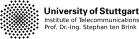
\includegraphics[width=0.9\textwidth]{img/logo_bitmap_example}
    \end{figure}

    \begin{itemize}
      \item Bitmaps are bad

        \begin{itemize}
          \item Do not scale very well
          \item Bad for high-resolution reprints
        \end{itemize}
      \item Use high resolution if bitmap is not avoidable
    \end{itemize}
  \end{columns}

\end{frame}

\begin{frame}{Comparison}

  \begin{columns}[t]

    \column{0.5\textwidth}

    \textbf{Method 1}

    \begin{itemize}
      \item Has some real advantages
      \item But also some disadvantages

        \begin{itemize}
          \item Which is bad
          \item But not so bad
        \end{itemize}
      \item Could be used for our research
    \end{itemize}

    \column{0.5\textwidth}

    \textbf{Method 2}

    \begin{itemize}
      \item Covers different topics

        \begin{itemize}
          \item Such as this topic
          \item And the other topic
        \end{itemize}
      \item Is not investigated by our research
    \end{itemize}
  \end{columns}

\end{frame}

\begin{frame}{Comparison Using Two Boxes}

  \begin{columns}[t]

    \column{0.4\textwidth}
    \begin{exampleblock}{advantages \cite{IEEE:15/0609r2}}

      \begin{itemize}
        \item advantage 1
        \item advantage 2
        \item advantage 3
        \item advantage 4
        \item advantage 5
      \end{itemize}
    \end{exampleblock}

    \column{0.0\textwidth}

    \column{0.4\textwidth}
    \begin{alertblock}{disadvantages}

      \begin{itemize}
        \item disadvantage 1
        \item disadvantage 2
        \item disadvantage 3
        \item disadvantage 4
        \item disadvantage 5
      \end{itemize}
    \end{alertblock}
  \end{columns}

  \bigskip{}

  $\mathit{\Longrightarrow}$ It is always a trade-off between the advantages
  and disadvantages of a certain method \cite{Jones:2015}
\end{frame}

\begin{frame}{Julia Plots}

  \begin{itemize}
    \item Julia supports direct export into PDF ({*}.PDF)
    \item Mention the main simulation parameters
    \item Take care that the font is large enough
  \end{itemize}
  \begin{figure}
    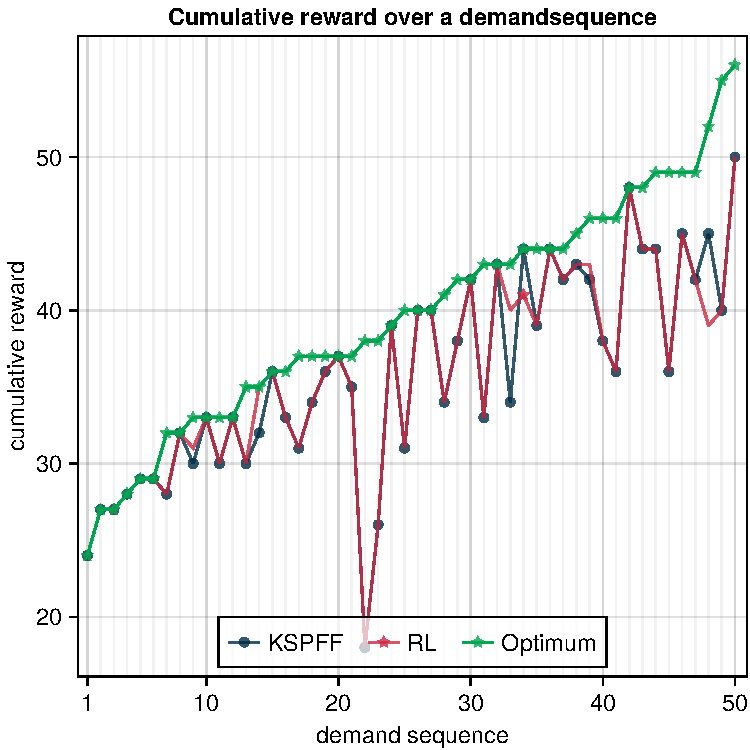
\includegraphics[width=0.45\textwidth]{img/rewards_unscaled.pdf}
  \end{figure}

\end{frame}

\begin{frame}{Using Blocks and Itemize Together}

  \begin{block}<1->{Testblock}

    \begin{itemize}
      \item Untitled block

        \begin{itemize}
          \item Subitem
        \end{itemize}
      \item Shown on all slides
    \end{itemize}
  \end{block}

  \begin{block}<2->{Some Example Block Title}

    \begin{itemize}
      \item $e^{i\pi}=-1$
      \item $e^{i\pi/2}=i$
      \item Only visible on the second slide
    \end{itemize}
  \end{block}
\end{frame}
\begin{frame}{Using Textblock}

  \begin{textblock}{5}(4,4)
    Text can be positioned freely with the textblock environemnt
  \end{textblock}
  \TPoptions{showboxes=true}
  \begin{textblock}{7}(1,7)
    \begin{tcolorbox}
      Boxes can be shown with \mint{latex}{\TPoptions{showboxes=true}}
    \end{tcolorbox}
  \end{textblock}
\end{frame}

\begin{frame}{Important Equations}

  \begin{block}{Attenuation Coefficient}

    \begin{align}
      \alpha\left(\omega\right) &
      =\frac{1}{\sqrt{2}}\sqrt{\sqrt{\left(R^{\prime2}+\omega^{2}L^{\prime2}\right)\left(G^{\prime2}+\omega^{2}C^{\prime2}\right)}+R^{\prime}G^{\prime}-\omega^{2}L^{\prime}C^{\prime}}\label{eq:att_coeff}
    \end{align}

  \end{block}

  \begin{block}{Reflection Coefficient}

    \begin{equation}
      r_{\mathrm{i}}=\frac{Z_{\mathrm{i}}-Z{}_{\mathrm{L}}}{Z_{\mathrm{i}}+Z{}_{\mathrm{L}}}
    \end{equation}

  \end{block}
  \begin{itemize}
    \item Use numbering for questions from the audience
    \item Avoid too many equations in your presentation
    \item (\ref{eq:att_coeff}) contains many unknown paramters
  \end{itemize}
\end{frame}

\begin{frame}{Tikz}

  \begin{center}
    \begin{figure}
      \scalebox{0.75}{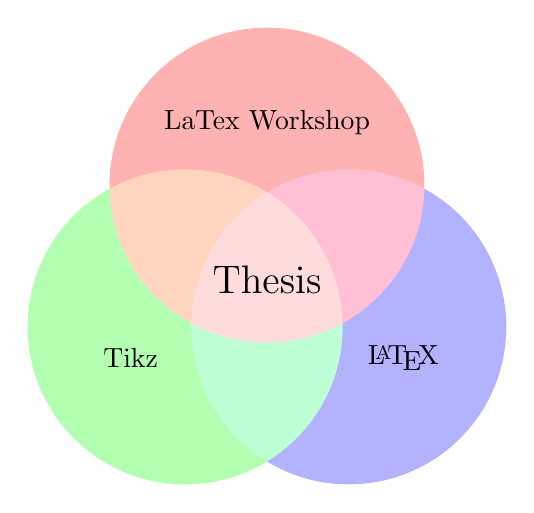
\begin{tikzpicture}
  \begin{scope}[blend group = soft light]
    \fill[red!30!white]   ( 90:1.2) circle (2);
    \fill[green!30!white] (210:1.2) circle (2);
    \fill[blue!30!white]  (330:1.2) circle (2);
  \end{scope}
  \node at ( 90:2)    {LaTex Workshop};
  \node at ( 210:2)   {Tikz};
  \node at ( 330:2)   {\LaTeX};
  \node [font=\Large] {Thesis};
\end{tikzpicture}
}
    \end{figure}
    \par
  \end{center}
  \begin{block}{Use Tikz}

    \begin{itemize}
      \item Many examples on texample.net/tikz
      \item Your results are innovative
      \item Figures can be easily included with the \textit{input} command
    \end{itemize}
  \end{block}
\end{frame}

\begin{frame}{Tikz (2)}

  \begin{block}{How to insert Tikz images:}

    \begin{itemize}
      \item Insert a figure float environment, remove the caption
        field (1x Backspace)
      \item Insert a preview box (last entry in the menu ``Insert'') into the
        figure box
      \item Insert a child document containing your Tikz code. Take
        care to select
        ``Input'', not ``Include'' and to check the preview option
      \item If required, scale the image by putting the preview box
        into a scalebox
        using ERT
    \end{itemize}
  \end{block}
\end{frame}

\section{Results}
\begin{frame}{Results}

  \begin{center}
    \begin{figure}
      \scalebox{0.75}{\tikzstyle{block} = [draw,fill=mittelblau!25,minimum size=2em]
% diameter of semicircle used to indicate that two lines are not connected
\def\radius{.7mm} 
\tikzstyle{branch}=[fill,
   shape=circle,
   minimum size=3pt,
   inner sep=0pt]

    \tikzset{
    buffer/.style={
        draw,
        shape border rotate=90,
        regular polygon,
        regular polygon sides=3,
        fill=red,
        node distance=2cm,
        minimum height=4em
    }
}
\tikzset{
    *|/.style={
        to path={
            (perpendicular cs: horizontal line through={(\tikztostart)},
                                 vertical line through={(\tikztotarget)})
            % is the same as (\tikztostart -| \tikztotarget)
            % but just to be safe: http://tex.stackexchange.com/a/29781/16595
            -- (\tikztotarget) \tikztonodes
        }
    }
}
\begin{tikzpicture}

  %\node at (0, 0) (AP1)  {\textbullet};
  \node [draw, minimum width=1cm, minimum height=0.5cm ] (rect) at (-2, 0) (Device) {\shortstack{Sensor}};
  \node [draw, minimum width=1cm, minimum height=0.5cm ] (rect) at (2, 0) (Watch) {\shortstack{Device}};

  \node [buffer, draw, fill=white, inner sep=0pt, minimum size=10pt, rotate=90 ] at (0, -1) (ant1) {};
  \node [draw, minimum width=1cm, minimum height=0.5cm ] (rect) at (1.5, -1.5) (Scope) {\shortstack{Oscilloscope}};
  \node [draw, minimum width=1cm, minimum height=0.5cm ] (rect) at (6, -1.5) (PC) {\shortstack{Signal Processing\\Julia}};


\draw [thick,red ] ([shift=(-30:.5cm) ]-1.5,0) arc (-30:30:.5cm);
\draw [thick,red ] ([shift=(-30:1cm) ]-1.5,0) arc (-30:30:1cm);
\draw [thick,red ] ([shift=(-30:1.5cm) ]-1.5,0) arc (-30:30:1.5cm);
\draw [thick,red ] ([shift=(-30:2cm) ]-1.5,0) arc (-30:30:2cm);
\draw [thick,red ] ([shift=(-25:2.5cm) ]-1.5,0) arc (-25:30:2.5cm);

\path [>=latex, shorten <=5pt, shorten >=5pt ] (Scope.east) edge [->] node  [above] {{Dump}} (PC);
   \draw (ant1.south)++(-0.112, -5pt) -- ++(0, -0.325) -> (Scope.west);


  \node  at (9, -1.5) (end) {Data};

\path [>=latex, shorten <=5pt, shorten >=5pt ] (PC.east) edge [->] (end);


\end{tikzpicture}
}
    \end{figure}
    \par
  \end{center}
  \begin{alertblock}{Results}

    Show your results in a Block, to point out that:
    \begin{itemize}
      \item Your results are innovative
      \item Your results are well interpreted
    \end{itemize}
  \end{alertblock}
\end{frame}

\section{Summary}
\begin{frame}{Summary}

  \begin{itemize}
    \item Showed how to use the \alert{presentation template}
    \item \alert{Typical layouts} for slides have been shown including

      \begin{itemize}
        \item Tables
        \item Images
        \item Multiple columns
      \end{itemize}
    \item Alarm text style can be used to mark the \alert{important parts}
      in lengthy sentences\\
      $\mathit{\rightarrow}$ But in general: keep it short
  \end{itemize}
  \medskip{}

  \begin{itemize}
    \item Outlook

      \begin{itemize}
        \item Discuss new template-features with your supervisor
        \item Newest release available on
          \url{https://appsrv1:3000/nclshrnk/BeamerThemeIKRv3.git}
          \setbeamercolor{bibliography item}{fg=mittelblau}
        \item Some References:
          \cite{Kuo:1981,IEEE:14/1193r0,IEEE:15/0919r1,Jones:2015,Ling:2015,Yang:2015,Zhang:2015}
      \end{itemize}
  \end{itemize}
\end{frame}
\breadcrumbsoff

\begin{frame}[noframenumbering]{References}

  \vspace{-2.15em}
  \begin{multicols}{2}
    %\scriptsize\bibliographystyle{deIEEEtran}
    % \scriptsize\bibliographystyle{apalike}
    \setbeamertemplate{bibliography item}[text]

    {\scriptsize{}\bibliographystyle{apalike}
      \bibliography{Bib}
    }{\scriptsize\par}

  \end{multicols}

  \beginbackup
\end{frame}
\end{document}
